%! TEX root = 0-main.tex
\chapter{Phase Transitions}
A phase transition is is an abrupt change in a certain property of a material; ``analyticity'' is no longer applicable at the transition. There are two types of of transitions. \emph{First order} transitions are characterized by a discontinuous first derivative of free energy and a discontinuous change in a variable \(X\). A \emph{Second Order} transition has this discontinuity at a higher order derivative, and consequently has a continuous change in the variable \(X\).

\section{van der Waals Fluid}
A classical ideal gas has no phase transition; this is due to the lack of interactions between particles. By adding a potential, we can describe phase transitions. Typical potentials have repulsions at short ranges (Pauli repulson force from overlapping orbitals) and attraction at larger distances (dipole-dipole interactions). We begin by examining the Helmholtz Free Energy of a classical ideal gass:
\[F_{IG}(T,V,N)=-Nk_B T \left[\ln\left(\frac{V}{N}\right)+\frac{3}{2}\ln\left(k_B T\right)+X\right]\]
we can add additional terms to encapsulate the interactions. The effective volume is reduced due to the repulsion by a effective factor of \(b\) per particle, while an attraction energy that reduces the total energy is proportianal to the density of particles \(N/V\) and the number of particles \(N\) is approximated by \(aN^2/V\). Thus, the Free Energy becomes
\begin{equation}
	F_{vdW} = -Nk_BT\left[\ln\left(\frac{V-bN}N\right)+\frac{3}{2}\ln(k_BT) + X \right]-a\left(\frac{N^2}{V}\right)
\end{equation}
for positive constants \(a,b>0\).

Computing the derivatives of the Free energy wrt \(T,V\), we obtain the equations of state
\begin{subequations}
	\begin{align}
		P&=\frac{Nk_BT}{V-bN}-\frac{aN^2}{V^2}\\
		U&=\frac{3}{2}k_BT - \frac{a}{N^2}{V}
	\end{align}
\end{subequations}

\begin{aside}[Energy from vdW]
	The derivative gives:
	\begin{align*}
		S&=-\frac{1}{T}\left(F+\frac{aN^2}{V}\right)+\frac{3}{2}k_B\\
		 &=-\frac{1}{T}(U-TS)-\frac{aN^2V}{T}+\frac{3}{2}Nk_B\\
		 &= S -\frac{U}{T} -\frac{aN^2}{VT}+\frac{3}{2}Nk_B
		 U=\frac{3}{2}Nk_BT -\frac{aN^2}{V}
	\end{align*}
\end{aside}
Because surfaces and other interfaces are neglected, the vdW fluid is an extensive system.

At high temperatures, the vdW fluid approaches the behaviour of an ideal gas. However, it deviates from an ideal gas when the temperature decreases. At high temperature, a \(PV\) plot is monotonic decreasing, but at a critical temperature \(T_c\), the \(PV\) plot will have an inflection point
\[\left(\pder{P}{V}\right)_{T,N}=0 \qquad \qquad \left(\pder{^2P}{V^2}\right)_{T,N}\]
This inflection point is characterized with the following:
\begin{equation}
	V_c = 3bN \qquad \qquad P_c=\frac{a}{27b^2} \qquad \qquad k_B T_c = \frac{8a}{27b}
\end{equation}
These three values can be determined from two equations because only two are independent. They satisfy the relation
\begin{equation}
	\frac{P_cV_c}{Nk_BT_c}=\frac{3}{8}
\end{equation}

Normalizing the variables with \(\tilde V = V/V_c\) and so forth, the vdW equation can be rewritten:
\begin{equation}
	\left(\tilde P + 3\tilde {V}^{-2}\right)\left(3\tilde V -1\right) = 8\tilde T
\end{equation}

\break{}

\subsection{Instability}
If we plot \(PV\) for \(T<T_c\), we see that for a certain region, the volume increases in response to an increase in temperature; however, this violates the stability condition \(\kappa_T\geq 0\) we showed in the previous chapter. This section of the curve represents unphysical states. 

\begin{figure}[!htbp]
	\begin{center}
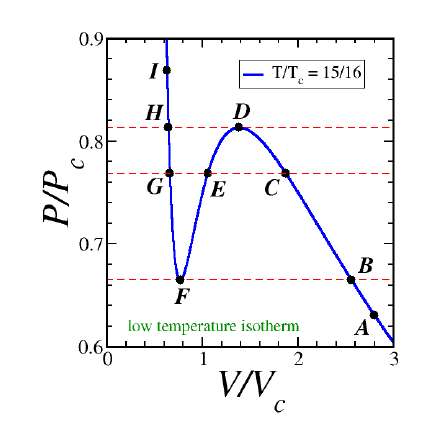
\includegraphics[scale=.7]{diagrams/phase/pv.png}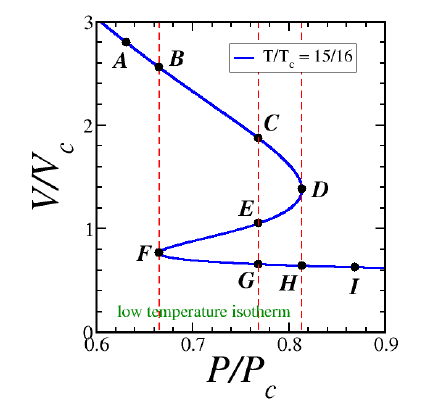
\includegraphics[scale=.7]{diagrams/phase/vp.png}
	\end{center}
	\caption{PV}\label{fig16:pv}
\end{figure}

Instead, we plot \(VP\), we get a triple-valued function in the region where \(\pder{V}{P}\geq0\).

Rewriting one of  the equations of state for the van der Waals fluid,
\begin{equation}
	(PV^2+aN^2)(V-bN)=Nk_BTV^2
\end{equation}
yields a cubic equation with three solutions. 
One of these solutions is the region of the curve where \(\pder{V}{P}\geq 0\); this we can discard as we know that it corresponds to an unstable state.
Instead we seek to replace this section with a different branch of the cubic.

As we want to vary pressure while holding temperature constant, we choose Gibbs free energy as a potential to study the system:
\[G=\mu N\]
As \(N\) remains constant, we seek to minimise \(\mu\). As the vdW fluid is extensive, we can use the Gibbs-Duhem relation
\[\d\mu =\cancelto{0}{-\left(\frac{S}{N}\right)\d{T}}+\frac{V}{N}\d{P}\]
Combining these two expressions,
\[G=\mu N = N\int\frac{V}{N}\d{P}=\int V\d{P}\]
Integrating numerically, we obtain the following graph of \(G_r = [G(P)-G(\frac{1}{3}P_c)]/(V_cP_c)\) against \(\tilde P\).

\begin{figure}[!htbp]
	\begin{center}
		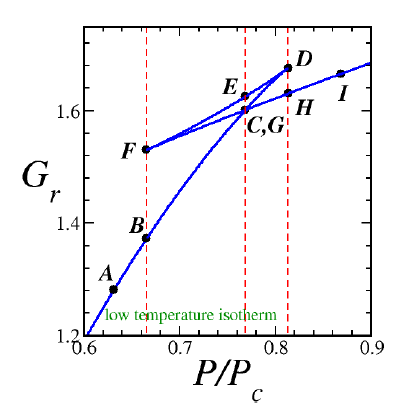
\includegraphics[scale=.6]{diagrams/phase/gp.png}
	\end{center}
	\caption{GP}\label{fig16:gp}
\end{figure}

Notice that the graph has a crossing point, at \(P\approx 0.76851\), and a closed loop.
The labelled points on the \(G_r\tilde P\) graph correspond to the same points on the \(\tilde V \tilde P\) graph, and show how \(G_r\) is built as \(V\) is integrated. The line CG is the pressure at which the graph crosses, and signifies the transition pressure for this system.

Recall that equilibria occur when \(G\) is minimized; because the loop lies above other portions of the graph, it is not at equilibrium. Thus, the ``real'' curve \(G\) is the curve in blue shown below

\begin{figure}[!htbp]
	\begin{center}
		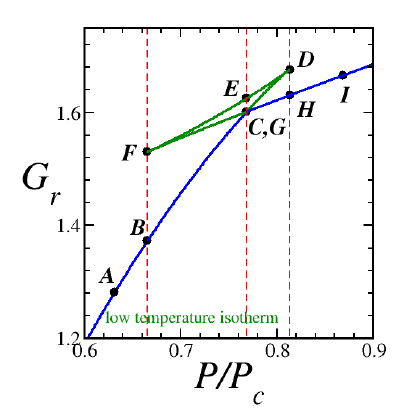
\includegraphics[scale=.65]{diagrams/phase/stab.png}
	\end{center}
	\caption{Stable}\label{fig16:stab}
\end{figure}

We already noted that the segment \(DF\) is unstable because it violates the stability condition. However, the sections \(CD\) and \(FG\) are long-lived \emph{metastable} states, which are stable to small fluctiations, but large fluctuations cause transitions. 

\subsection{Maxwell Construction}
While the Gibbs free energy may be obtained, the numerical calculation can be difficult to perform. Instead, the transition temperature may be obtained via the \emph{Maxwell construction}. Extending the line \(CG\) on the \(PV\) curve, the region bounded by \(CDE\) and by \(EFG\) actually have the same area! 

\begin{figure}[!htbp]
	\begin{center}
		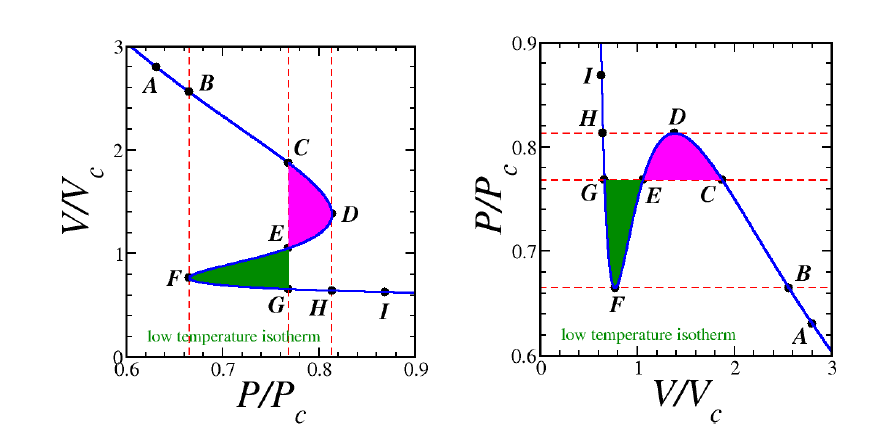
\includegraphics[scale=.7]{diagrams/phase/max.png}
	\end{center}
	\caption{Maxwell Construction}\label{fig16:max}
\end{figure}

This is because this integration follows a closed loop in \(GP\); because the starting \(G\)  must equal the final, the (signed) sum of the two areas must be zero. This area is conserved if we flip the axes, so we can instead compute \(P\d{V}\). Guessing \(P\), we can solve the cubic and obtain endpoints of integration, and adjust our guess according to the difference in the areas.

\subsection{Multiple Phases}
Note that points \(C\) and \(G\) exist at the same pressure and at the same Free Energy, but have different volumes; there exists two stable configurations of the fluid at this pressure. Point \(G\), having a lower volume, corresponds to a liquid phase, while point \(C\) with the greater volume corresponds to a gas. Repeating the maxwell construction for different isotherms, we can determine the transition pressure as a function of temperature.
	
Plotting the temperature against the volumes of the two phases at the transition, we obtain the below graph. The point at the top of the curve is the \emph{critical point}, characterized by \(T_c, V_c, P_c\), and the meta-stable states are so-called ``spinodals,'' characterized by points \(D\) and \(F\). 

\begin{figure}[!htbp]
	\begin{center}
		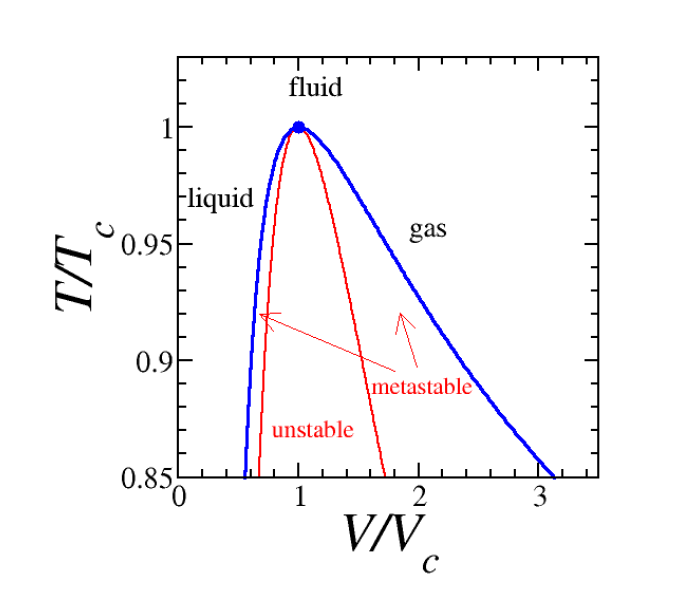
\includegraphics[scale=.4]{diagrams/phase/meta.png}
	\end{center}
	\caption{idk}\label{fig16:meta}
\end{figure}

If we instead plot the pressure against the temperature, we get obtain the familiar phase diagram. Above \(T_c\), there is no distinction between liquid and gas; they form a uniform ``fluid.'' In fact, you can go smoothly from gas to liquid by going around the critical point. The blue line in the phase diagram is known as the \emph{coexistence curve}.

\begin{figure}[!htbp]
	\begin{center}
		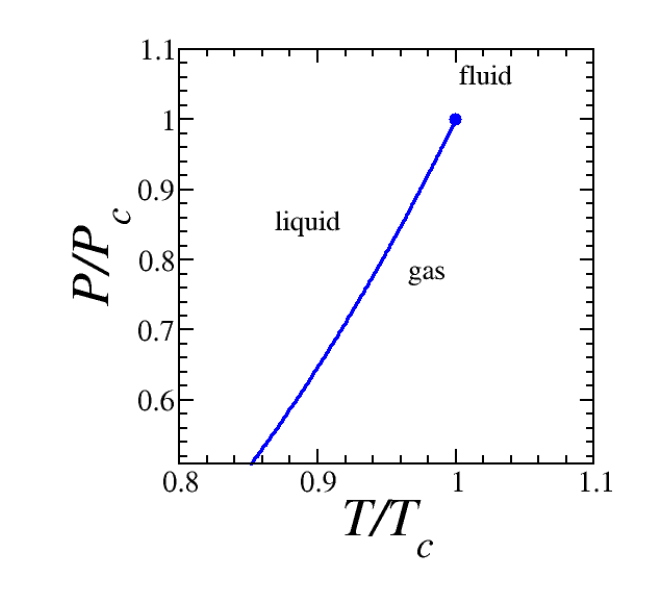
\includegraphics[scale=.4]{diagrams/phase/phase.png}
	\end{center}
	\caption{Phase Diagram}\label{fig16:phase}
\end{figure}

\section{Helmholtz Free energy}
Rewiting the helmholtz free energy in terms of dimensionless quantities,
\begin{equation}
	F_r = \frac{F_{vdW}}{V_cP_c} = -\frac{8}{3}\tilde T \left[\ln\left(3\tilde V-1\right)+\frac{3}{2}\ln\left(\tilde T\right)+\tilde X\right]-\frac{3}{\tilde V}
\end{equation}
The second derivative is then
\begin{equation}
	\left(\pder{^2F_r}{\tilde V^2}\right)_{\tilde T, N}=\frac{24\tilde T}{(3\tilde V-1)^2}-\frac{6}{\tilde V^3}
\end{equation}
Because this quantity is related to the isothermal compresssibility, it must be positive. If we plot this second derivative against volume for an isotherm, we will see that below the critical temperaure, there is a region where graph goes below zero. The intercepts are the volumes of the liquid and gas respecively, and are connected by a straight \(F''=0\) line. 

\diagram{}

\section{Latent Heat}
Energy is required to cross the coexistence curve to go from a liquid to a gas. This energy is known as the \emph{latent heat of vaporisation}. We can obtain the latent heat by examining the entropy.  Along an isotherm, the change in entropy is given
\[\d{S} = \left(\pder{S}{V}\right)_{T,V}\d{V}\]
Using the maxwell relation
\[\left(\pder{S}{V}\right)_{T,N}=\left(\pder{P}{T}\right)_{V,N}=\frac{Nk_B}{V-bN}\]
we obtain
\[\Delta S = Nk_B\int_{V_\text{liquid}}^{V_\text{gas}}\frac{\d{V}}{V-bN}\]
thus, along the isotherm, the change in heat is
\[\Delta Q = T\Delta S\]
The latent heat per particle is defined to be the \emph{latent heat} of the transition
\begin{equation}
	\ell = \frac{T\Delta S}{N}
\end{equation}
and the total energy to complete the transition is the \emph{heat capacity} of the transition.
\begin{equation}
	L=N\ell=T\Delta S
\end{equation}

\section{Clausius-Clapeyron Equation}
The Clausius-Clapeyron Equation relates the slope of the coexistence curve with the volume change and latent heat of the transition.

Let \(X,Y\) denote the liquid phase at two points along the coexistence curve, and \(X',Y'\) denote the gas phase at the corresponding points along the coexistence curve. The pairs \(X,X'\) and \(Y,Y'\) are very close, so \(\d{T} = \d{T'}\) and \(\d{P} = \d{P'}\).

Further, because the liquid and gas phase are at equilibrium, \(\mu_X = \mu_{X'}\) and similarly at \(Y\). Using Gibbs-Duhem and the same \(N\) number of particles for both transitions,
\[\d\mu = -\frac{S}{N}\d{T}+\frac{V}{N}\d{P}\]
\[\d{\mu'} = -\frac{S'}{N}\d{T}+\frac{V'}{N}\d{P}\]
Because these two equations are equal, we can obtain:
\[\der{P}{T}=\frac{S'-S}{V'-V}=\frac{\Delta S}{\Delta V} = \frac{T\Delta S}{T\Delta V}\]
\begin{equation}
	\der{P}{T}=\frac{L}{T\Delta V}
\end{equation}
where \(\Delta V\) is the volume change of the transition. The Clausius-Claperyron equation is a genral equation for any phase transition. Note that \(L>0\) and, for most materials, \(\Delta V=0\). A notable exception is water, which has \(\Delta V<0\), which is why ice floats.

\section{Gibb's Phase Rule}
Gibb's phase rule limits the structures allowed in phase diagrams. It specifies the number  of independent variables  \(F\) of a coexistence structure---\(F=0\) provides a point, \(F=1\) provides a line, \(F=2\) provides a surface, and so forth. The rule is given by
\begin{equation}
	F = K - \phi + 2
\end{equation}
where \(K\) is the number of components (e.g.\ chemical species) and \(\phi\) is the number of coexisting phases.

Let \(x_k^{(j)}\) denote the concentrations (mole fraction) of component \(k\) in phase \(j\):
\[\{x_k^{(j)}=N_k^{(j)}/N^{(j)} \vert k=1,\ldots,K\}\]
where
\[N^{(j)}=\sum_kN_k^{(j)}\]
is the total number of all species in phase \(j\). The concentrations of any given phase must be one:
\begin{equation}
	\sum_kx_k^{(j)}=1
\end{equation}
which follows immediatly on the definition of \(x_k^{(j)}\). The number of independent \(x_k^{(j)}\) is then \(K-1\) which gives a total number of variables of \(P\), \(V\) and \(\phi *(K-1)\), giving
\(2+\phi*(K-1)\) variables, which may or may not be independent.

Because the \(\phi\) phases are all in equilibrium (by virtue of coexisting), we further have the \(\phi-1\) constraints:
\[\mu_k^{(1)}=\cdots=\mu_k^{(\phi)}\]
for each component\(K\), yielding \(K(\phi-1)\) total constraints. Subtracting from the total number of variables,
\[F=2+\phi*(K-1)-K(\phi-1)=2+K-\phi\]

For example, for water, at the ice-water transition, we have 
\[F=2+(K=1)-(\phi=2)=1\]
as there is only 1 component (\ce{H2O}), but two coexistant phases.


